\section{Study region and data}
\label{sec:data}

\subsection{Region}
The study region is Trøndelag--Dovre in central Norway, within \SI{170}{km} of \ang{63.2}\,N, \ang{10.0}\,E (Fig.~\ref{fig:map-no}). It spans the outer coast with islands and skerries, the Trondheimsfjord, forested valleys and the Dovre mountain plateau above \SI{1000}{m}; the roads follow valleys and fjords, so that the region contains open coastal roads, forest corridors, valley roads and mountain passes within a few hours' drive. This variety of road environments is the reason for choosing it.

\begin{figure}[!htbp]
\centering
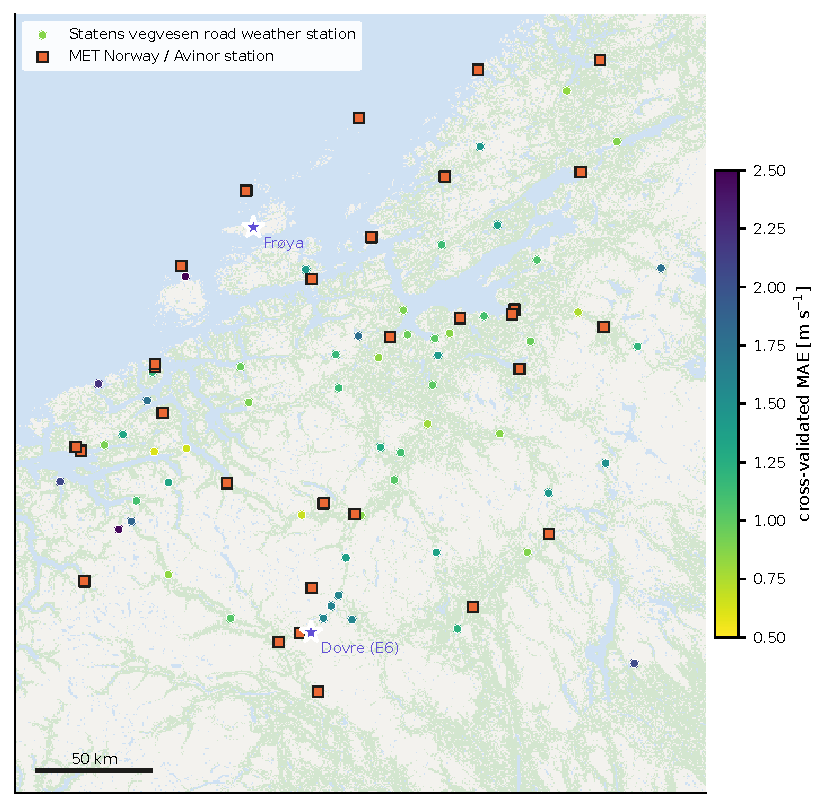
\includegraphics[width=\textwidth]{figures/fig01_norway_area.pdf}
\caption{Study region: reference stations of MET Norway and Avinor (squares), road weather stations of Statens vegvesen (circles, coloured by the cross-validated mean absolute error of the corrected hourly wind speed) and the two road sections with vehicle measurements (stars). Background: forest, open land and water from ESA WorldCover.}
\label{fig:map-no}
\end{figure}

\subsection{Reference stations}
The reference network consists of the \noRef{} stations of MET Norway and Avinor (airports) in the region that report hourly wind at \SI{10}{m}, obtained from the Frost API of MET Norway \citep{Frost}. The year 2023 was used only to estimate the site factors of the reference stations (Section~\ref{sec:methods}).

\subsection{Roadside stations}
Statens vegvesen road weather stations report 10-min wind, distributed through Frost with a nominal sensor level of \SI{10}{m} above ground; on-the-hour values from \noStart{} to \noEnd{} (\noHours{} hours) were used. Speeds were checked for implausible values ($>\SI{60}{m.s^{-1}}$) and stuck sensors (the same non-zero value in six or more consecutive hours, or zero in twelve or more), which removed \noQcPct\,\% of the values; the \noTrv{} stations with at least 2000 valid hours were retained.

\subsection{Geodata}
Object heights were taken from airborne laser scanning, as the difference between the national digital surface and terrain models of Kartverket \citep{Kartverket}, resampled to \SI{10}{m}; objects higher than \SI{5}{m} are counted as trees or obstacles. Open water was taken from ESA WorldCover \citep{WorldCover}. The road axis at each roadside station was obtained by snapping the station to the OpenStreetMap road network with OSRM \citep{Luxen2011}.

\subsection{Vehicle measurements}
The NOR-XWIND data set \citep{NORXWIND} contains wind measured with an ultrasonic anemometer on a van (sensor \SI{3.4}{m} above ground) together with high-rate GNSS and inertial data \citep{Reymert2025}. Two road sections lie in the region: the E6 across the Dovre mountains (2020-10-29 and 2020-10-31) and the open coast of Frøya (2020-11-05). The anemometer orientation and gain were calibrated with the consistency of opposite driving directions, and the ground-fixed wind was averaged over road segments. There are \vehN{} segment passages (\vehNDovre{} at Dovre, \vehNFroya{} at Frøya), but they fall in only \vehHours{} distinct hours (\vehHoursDovre{} and \vehHoursFroya{}), so that the vehicle validation is a case study rather than a statistical test. The MET Nordic analysis \citep{MetNordic,Nipen2020}, a post-processed product of the MetCoOp ensemble prediction system \citep{Muller2017}, was interpolated to the segments and is used as an independent benchmark.

\subsection{Independent check region}
To test whether the findings hold in a different landscape, the same analysis was repeated in a flat-to-hilly, forest-dominated region within \SI{120}{km} of road RV40 between Gothenburg and Borås in western Sweden, with \seRef{} synoptic stations of SMHI \citep{SMHIopen} and \seTrv{} Trafikverket road weather stations at \SI{6}{m} \citep{TRVapi}. Because the Trafikverket API keeps only seven days, this record covers \seHours{} hours in November 2026. Object heights came from the NMD layer of Naturvårdsverket \citep{NMD}. Details are given in \ref{app:sweden}; the main text reports the Swedish results only where they confirm or contradict the Norwegian ones.
